%%%%%%%%%%%%%%%%%%%%%%%%%%%%%%%%%%%%%%%%%%%%%%%%%%%%%%%%%%%%%%%%%%%%%%%%%%%%%%%%%%%%%%
%%%%%%%%%%%%%%%%%%%%%%%%%%%%%%%%%% Settings %%%%%%%%%%%%%%%%%%%%%%%%%%%%%%%%%%%%%%%%%%
%%%%%%%%%%%%%%%%%%%%%%%%%%%%%%%%%%%%%%%%%%%%%%%%%%%%%%%%%%%%%%%%%%%%%%%%%%%%%%%%%%%%%%

\documentclass{beamer}
\usepackage[utf8]{inputenc}
\usepackage[english]{babel}
\usepackage[T1]{fontenc}
\usepackage{subfig}
\usepackage{appendixnumberbeamer}

\usefonttheme{professionalfonts}
\usepackage{mathspec}
\setsansfont[BoldFont={Fira Sans},
Numbers={OldStyle}]{Fira Sans Light}
\setmathsfont(Digits)[Numbers={Lining, Proportional}]{Fira Sans Light}

\def\mytitle{Solving the Harvest CPR \\Appropriation Problem with \\Policy Gradient Techniques}
\def\mysubtitle{AAS Final Project - Academic Year 2020/2021}
\def\myshortfullname{A. Falai}
\def\myfullname{Alessio Falai}
\def\myemail{alessio.falai@studio.unibo.it}
\def\myshortinstitute{UNIBO}
\def\myinstitute{Alma Mater Studiorum - University of Bologna}
\title{\mytitle}
\subtitle{\mysubtitle}
\author[\myshortfullname]{\myfullname \newline \texttt{\myemail}}
\date{\today}
\institute[\myshortinstitute]{\myinstitute}
\titlegraphic{\hfill
\includegraphics[height=1.5cm]{../assets/unibo-logo.eps}}

\usetheme[progressbar=frametitle, numbering=none, background=light, titleformat=smallcaps, block=fill]{metropolis}
\useoutertheme{metropolis}
\useinnertheme{metropolis}
\usefonttheme{metropolis}
\usecolortheme{metropolis}
\setbeamercovered{dynamic}
\setbeamercolor{background canvas}{bg=white}

% Edit progressbar width
\makeatletter
\setlength{\metropolis@progressinheadfoot@linewidth}{1.5pt}
\setlength{\metropolis@progressonsectionpage@linewidth}{1.5pt}
\makeatother

% Change shape size for itemize
\setbeamertemplate{itemize item}[circle]
\setbeamertemplate{itemize subitem}[square]

%%%%%%%%%%%%%%%%%%%%%%%%%%%%%%%%%%%%%%%%%%%%%%%%%%%%%%%%%%%%%%%%%%%%%%%%%%%%%%%%%%%%%%
%%%%%%%%%%%%%%%%%%%%%%%%%%%%%%%%%% Document %%%%%%%%%%%%%%%%%%%%%%%%%%%%%%%%%%%%%%%%%%
%%%%%%%%%%%%%%%%%%%%%%%%%%%%%%%%%%%%%%%%%%%%%%%%%%%%%%%%%%%%%%%%%%%%%%%%%%%%%%%%%%%%%% 

\begin{document}

%%%%%%%%%%%%%%%%%%%%%%%%%%%%%%%%%%%%%%%%%%%%%%%%%%%%%%%%%%%%%%%%%%%%%%%%%%%%%%%%%%%%%%
%%%%%%%%%%%%%%%%%%%%%%%%%%%%%%%%% Title & TOC %%%%%%%%%%%%%%%%%%%%%%%%%%%%%%%%%%%%%%%%
%%%%%%%%%%%%%%%%%%%%%%%%%%%%%%%%%%%%%%%%%%%%%%%%%%%%%%%%%%%%%%%%%%%%%%%%%%%%%%%%%%%%%% 

\renewcommand*{\insertpagenumber}{%
	\Roman{framenumber}%
}%
\makeatother
\setbeamertemplate{footline}
{
  \leavevmode%
  \hbox{%
  \begin{beamercolorbox}[wd=.3\paperwidth,ht=2.25ex,dp=1ex,center]{author in head/foot}%
    \usebeamerfont{author in head/foot}\insertshortauthor ~ (\myshortinstitute)
  \end{beamercolorbox}%
  \begin{beamercolorbox}[wd=.6\paperwidth,ht=2.25ex,dp=1ex,center]{block title}%
    \usebeamerfont{title in head/foot}\insertshorttitle
  \end{beamercolorbox}%
  \begin{beamercolorbox}[wd=.1\paperwidth,ht=2.25ex,dp=1ex,center]{block body}%
    \insertpagenumber{} \hspace*{1ex}
  \end{beamercolorbox}}%
  \vskip0pt%
}
\makeatletter
\setbeamertemplate{navigation symbols}{}

\begin{frame}
	\maketitle
\end{frame}

%%%%%%%%%%%%%%%%%%%%%%%%%%%%%%%%%%%%%%%%%%%%%%%%%%%%%%%%%%%%%%%%%%%%%%%%%%%%%%%%%%%%%%
%%%%%%%%%%%%%%%%%%%%%%%%%%%%%%%%% Main content %%%%%%%%%%%%%%%%%%%%%%%%%%%%%%%%%%%%%%%
%%%%%%%%%%%%%%%%%%%%%%%%%%%%%%%%%%%%%%%%%%%%%%%%%%%%%%%%%%%%%%%%%%%%%%%%%%%%%%%%%%%%%% 

\setcounter{framenumber}{0}
\makeatother
\setbeamertemplate{footline}
{
  \leavevmode%
  \hbox{%
  \begin{beamercolorbox}[wd=.3\paperwidth,ht=2.25ex,dp=1ex,center]{author in head/foot}%
    \usebeamerfont{author in head/foot}\insertshortauthor ~ (\myshortinstitute)
  \end{beamercolorbox}%
  \begin{beamercolorbox}[wd=.6\paperwidth,ht=2.25ex,dp=1ex,center]{block title}%
    \usebeamerfont{title in head/foot}\insertshorttitle
  \end{beamercolorbox}%
  \begin{beamercolorbox}[wd=.1\paperwidth,ht=2.25ex,dp=1ex,center]{block body}%
    \insertframenumber{} / \inserttotalframenumber\hspace*{1ex}
  \end{beamercolorbox}}%
  \vskip0pt%
}
\makeatletter
\setbeamertemplate{navigation symbols}{}

\begin{frame}
	\frametitle{Environment}
	\center
	\begin{columns}
		\begin{column}{0.6\textwidth}
			\begin{figure}
				\centering
				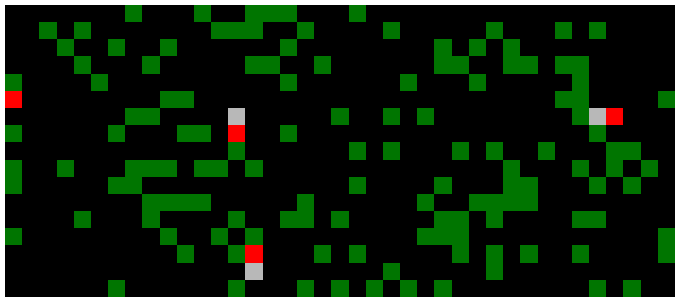
\includegraphics[width=0.7\linewidth]{../assets/env-example.png}
				\caption*{Full environment}
			\end{figure}
		\end{column}
		\begin{column}{0.4\textwidth}
			\begin{figure}
				\centering
				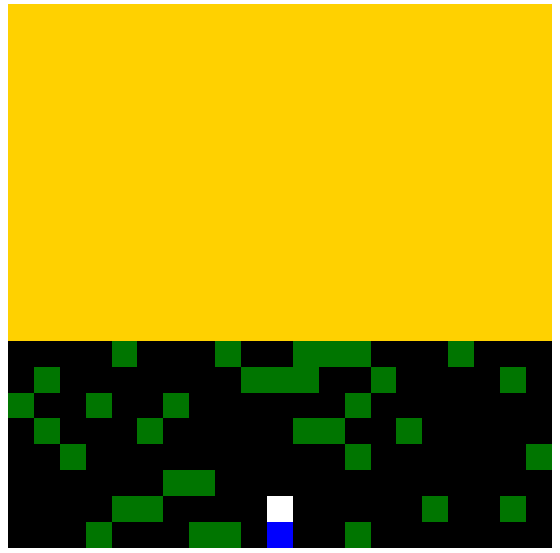
\includegraphics[width=0.7\linewidth]{../assets/obs-example.png}
				\caption*{Local observation}
			\end{figure}
		\end{column}
	\end{columns}
	\begin{itemize}
		\item Small $25\times 7$ grid for the single-agent setting and big $39\times 17$ map for multi-agent scenarios
		\item $9$ actions in total: movement + tagging + gifting
		\item Local observation: RGB image of size $3\times20\times21$ ($20$ squares ahead and $10$ squares on each side of the agent)
	\end{itemize}
\end{frame}

\begin{frame}
	\frametitle{Social Learning}
	\begin{itemize}
		\item Social Learning: reshape the reward function of other agents with the goal of promoting cooperation
		\item Gifting: peer-rewarding strategy in which agents can reward others with a new specialized action
		\item Gifting mechanisms: each time an agent sends a gift $g$, its gifting budget is decremented by $g$
		\begin{itemize}
			\item Zero-Sum: the budget is infinite, but the agent incurs a penalty $-g$ for every gifting action taken
			\item Fixed Budget: the budget is fixed at the start of the episode and when it's empty no more gifting can happen
			\item Replenishable Budget: the budget expands as a function of collected environmental rewards
		\end{itemize}
	\end{itemize}
\end{frame}

\begin{frame}
	\frametitle{Experiments}
	\begin{enumerate}
		\item Single-agent DQN vs VPG with RLlib
		\item Custom VPG vs TRPO vs PPO on Cartpole
		\item Custom VPG vs TRPO vs PPO on single-agent Harvest
		\item Custom PPO on multi-agent Harvest, with and without Zero-Sum gifting
		\item Custom PPO on multi-agent Harvest, with Replenishable and Fixed Budget gifting
	\end{enumerate}
\end{frame}


%%%%%%%%%%%%%%%%%%%%%%%%%%%%%%%%%%%%%%%%%%%%%%%%%%%%%%%%%%%%%%%%%%%%%%%%%%%%%%%%%%%%%%
%%%%%%%%%%%%%%%%%%%%%%%%%%%%%%%%%%% Appendix %%%%%%%%%%%%%%%%%%%%%%%%%%%%%%%%%%%%%%%%%
%%%%%%%%%%%%%%%%%%%%%%%%%%%%%%%%%%%%%%%%%%%%%%%%%%%%%%%%%%%%%%%%%%%%%%%%%%%%%%%%%%%%%% 

\appendix

\begin{frame}[standout]
	Thank you for your attention
\end{frame}

\begin{frame}
	\frametitle{References}
	\nocite{*}
    \bibliography{references}
    \bibliographystyle{plain}
\end{frame}

{
  \setbeamercolor{background canvas}{bg=alerted text.fg}
  \begin{frame}
    \centering \Large \textbf{\textsc{Backup frames}}
  \end{frame}
}

\begin{frame}
	\frametitle{Single-agent DQN vs VPG with RLlib}
	\begin{figure}
		\centering
		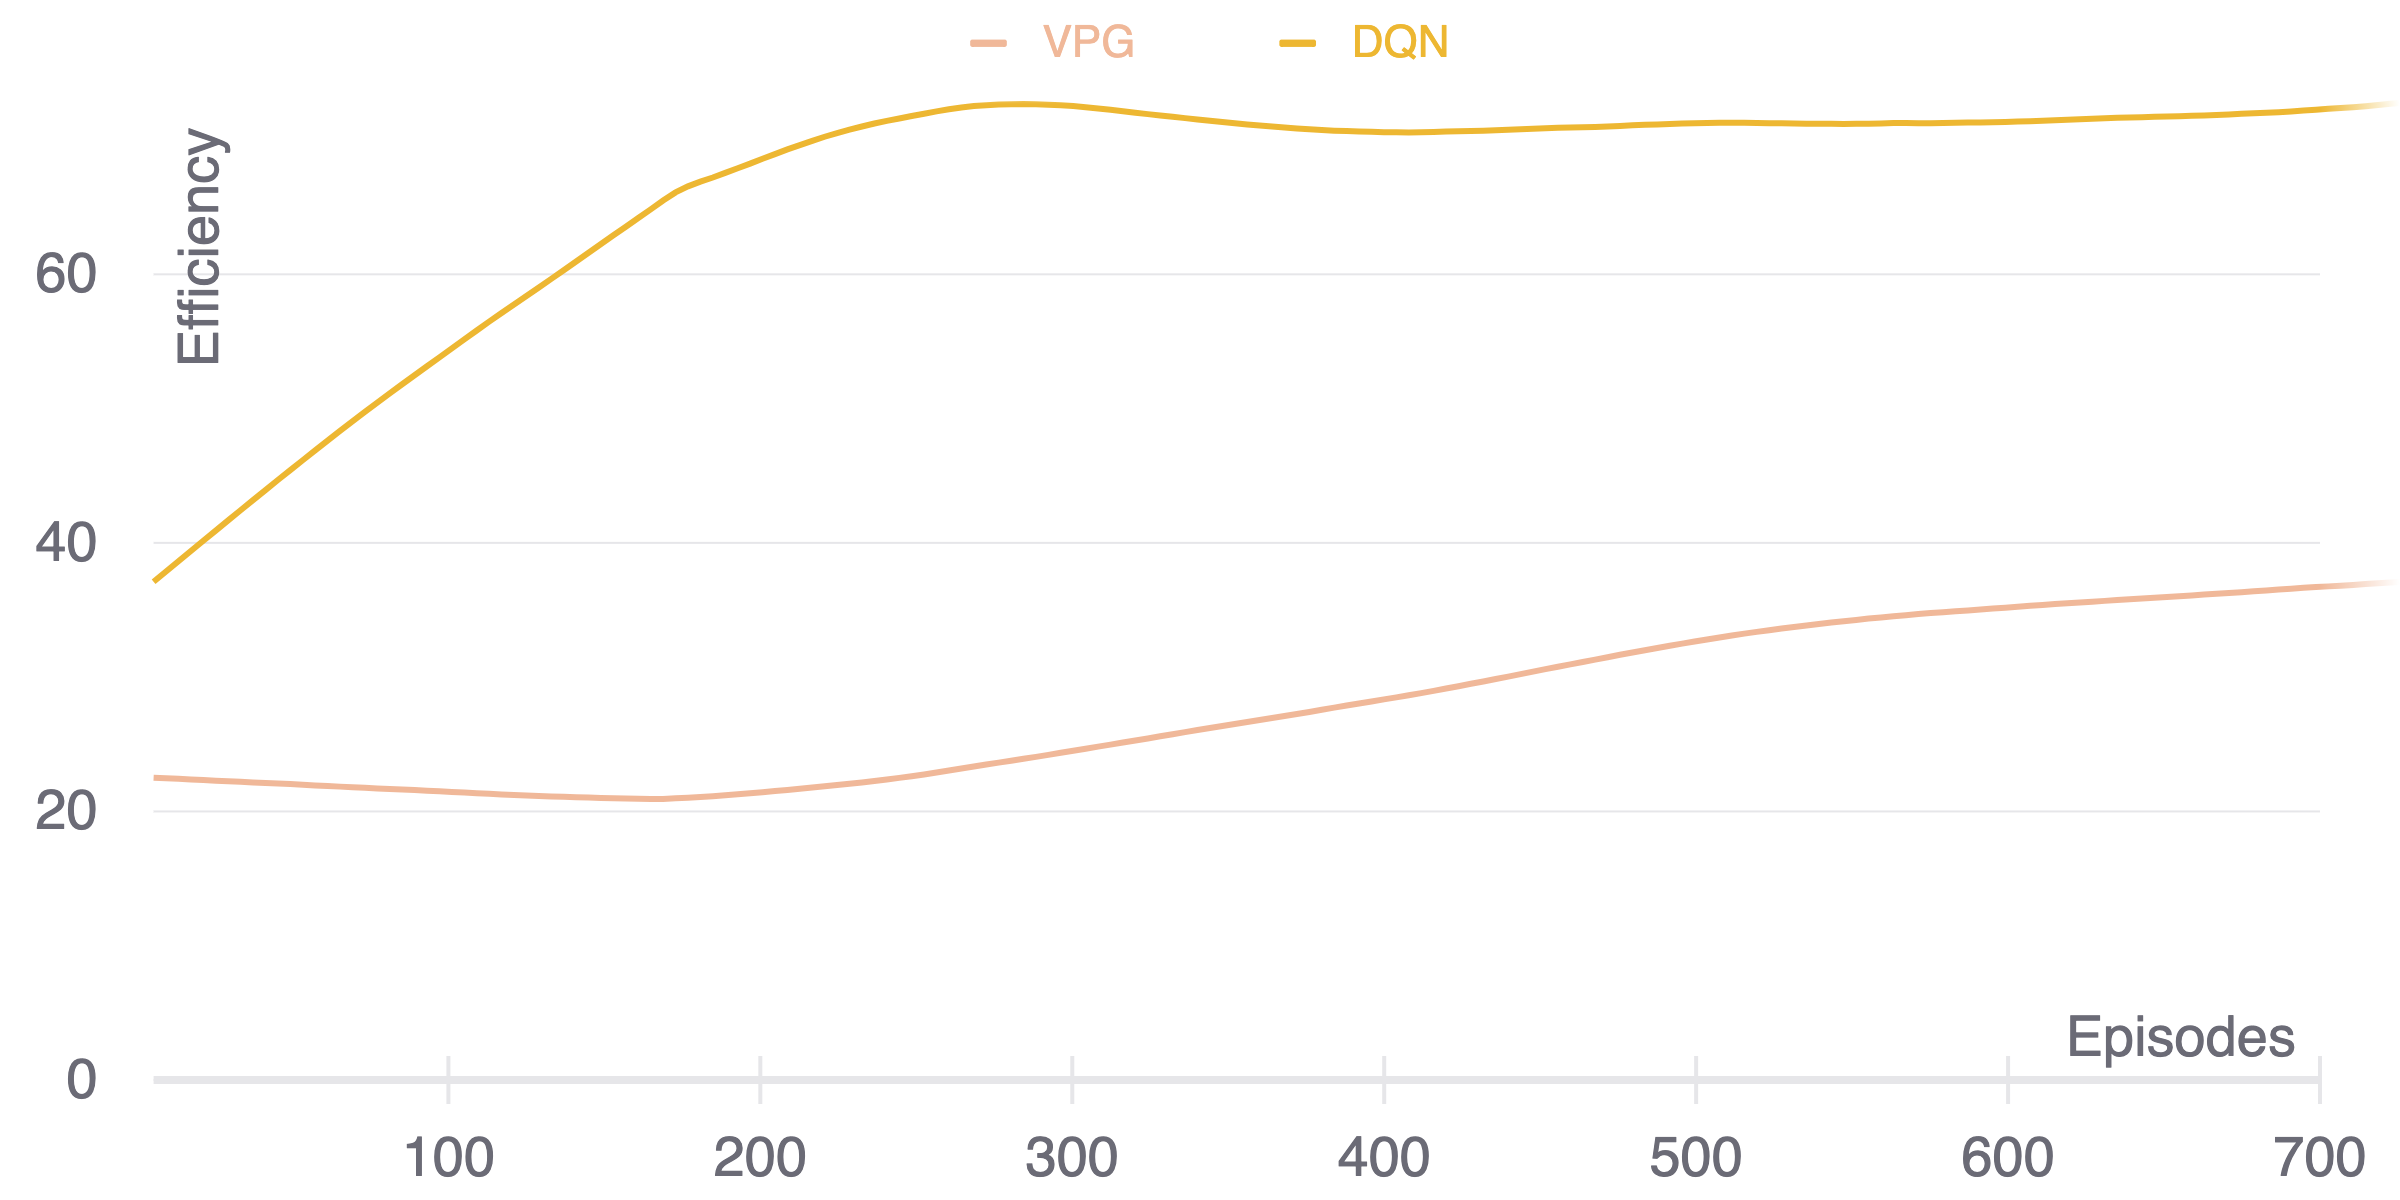
\includegraphics[width=0.9\linewidth]{../assets/dqn-vpg-rllib-single-efficiency.png}
		\caption*{Value-based methods seem more suited for the Harvest environment (higher returns)}
	\end{figure}
\end{frame}

\begin{frame}
	\frametitle{Custom VPG vs TRPO vs PPO on Cartpole}
	\begin{figure}
		\centering
		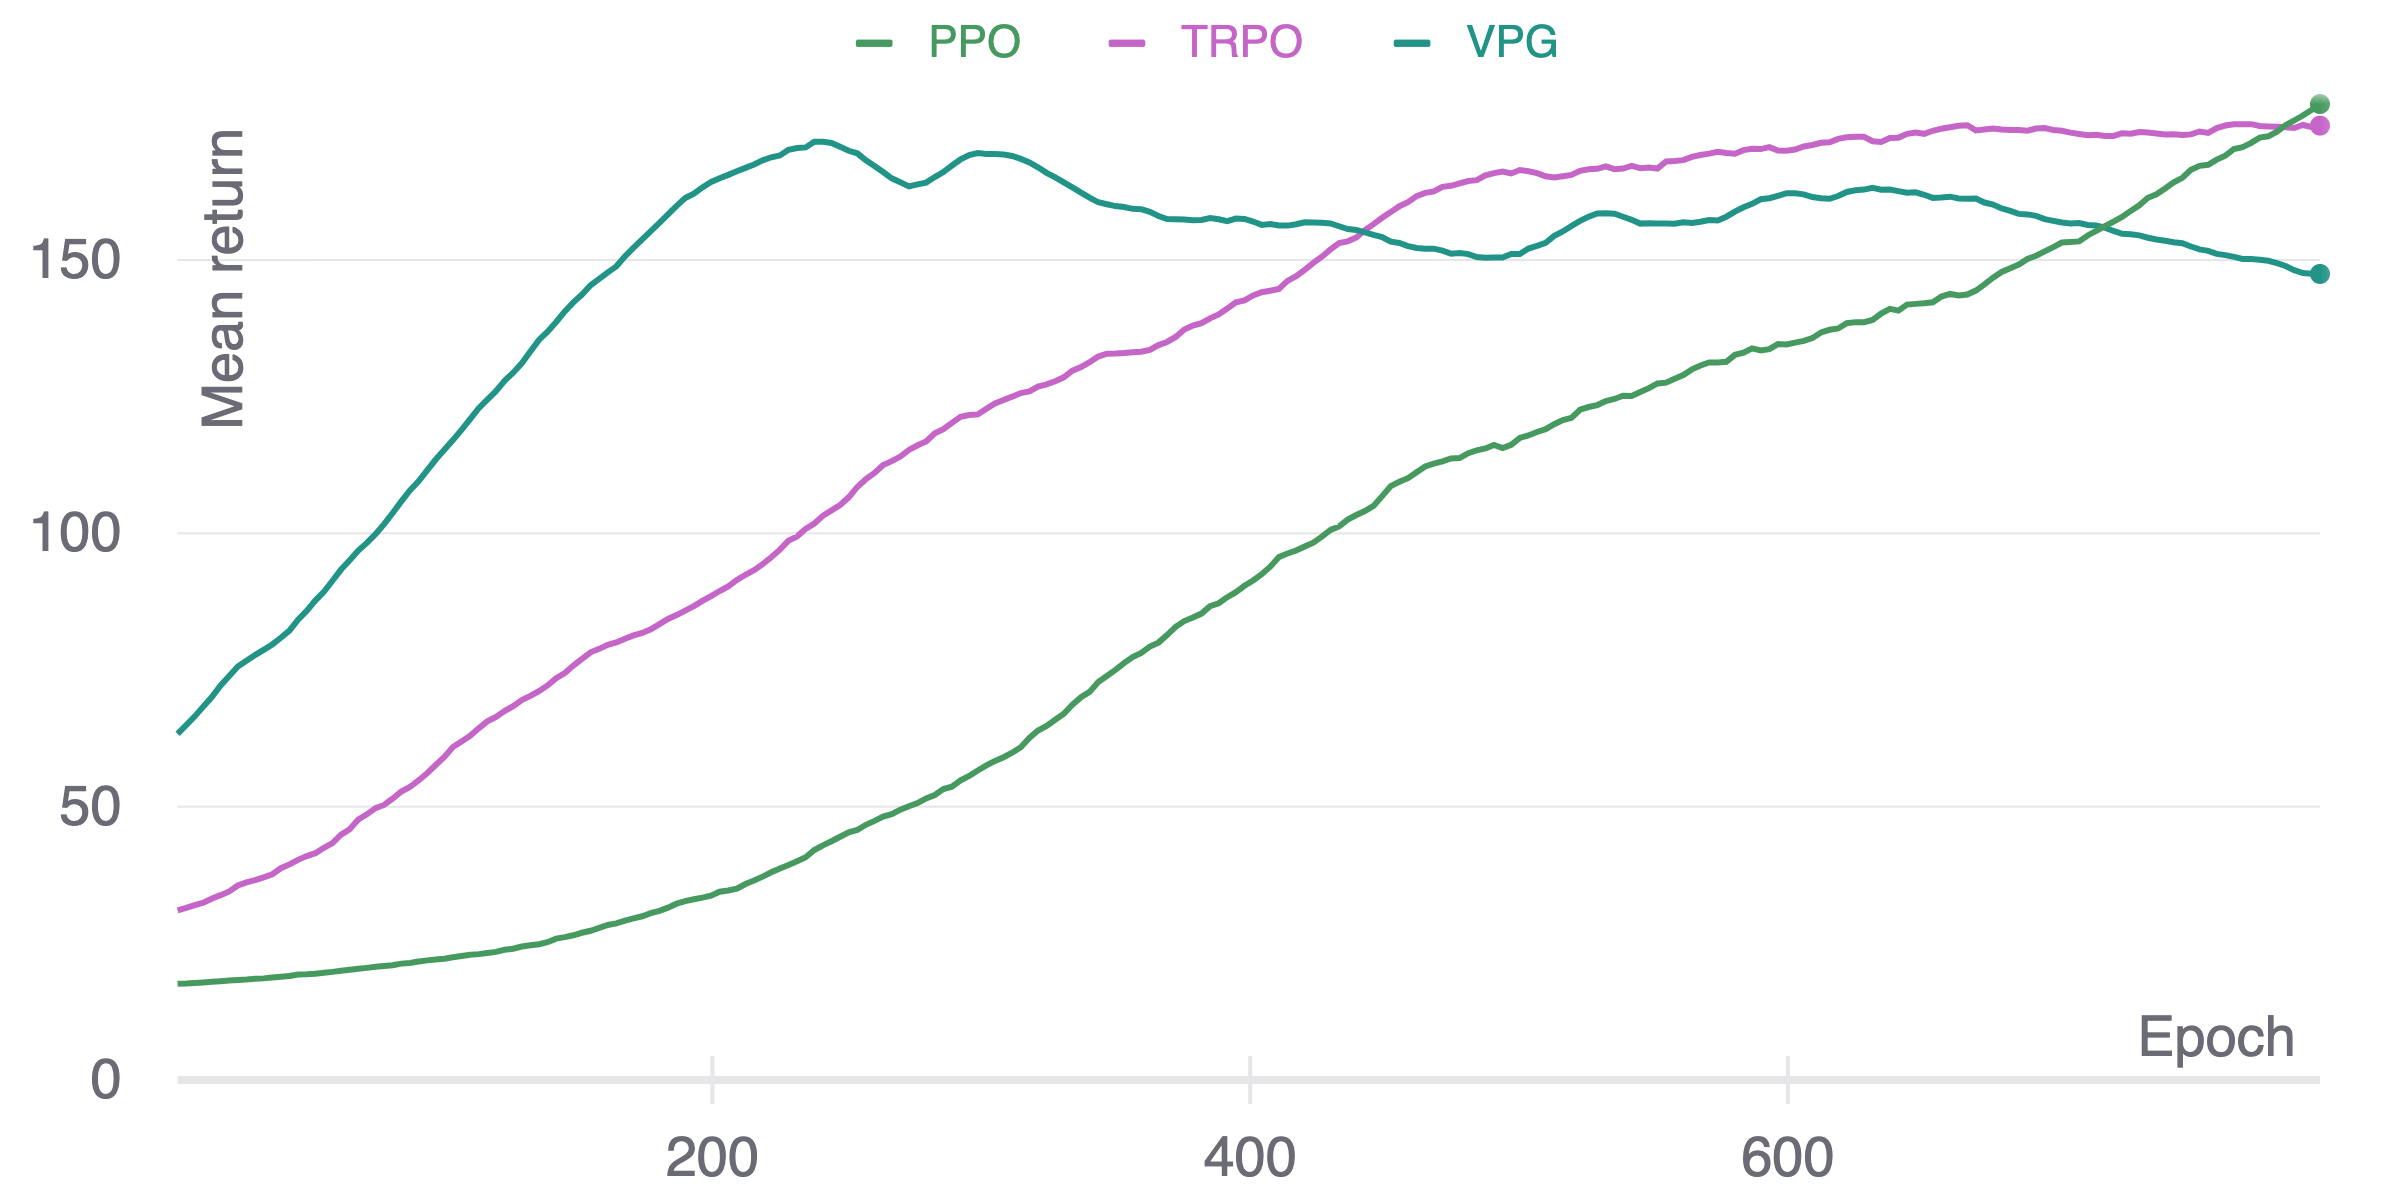
\includegraphics[width=0.9\linewidth]{../assets/cartpole-pg-return.png}
		\caption*{Custom implementations of policy gradient methods are valid, as all agents converge to good returns in the selected test environment}
	\end{figure}
\end{frame}

\begin{frame}
	\frametitle{Custom VPG vs TRPO vs PPO on single-agent Harvest}
	\begin{figure}
		\centering
		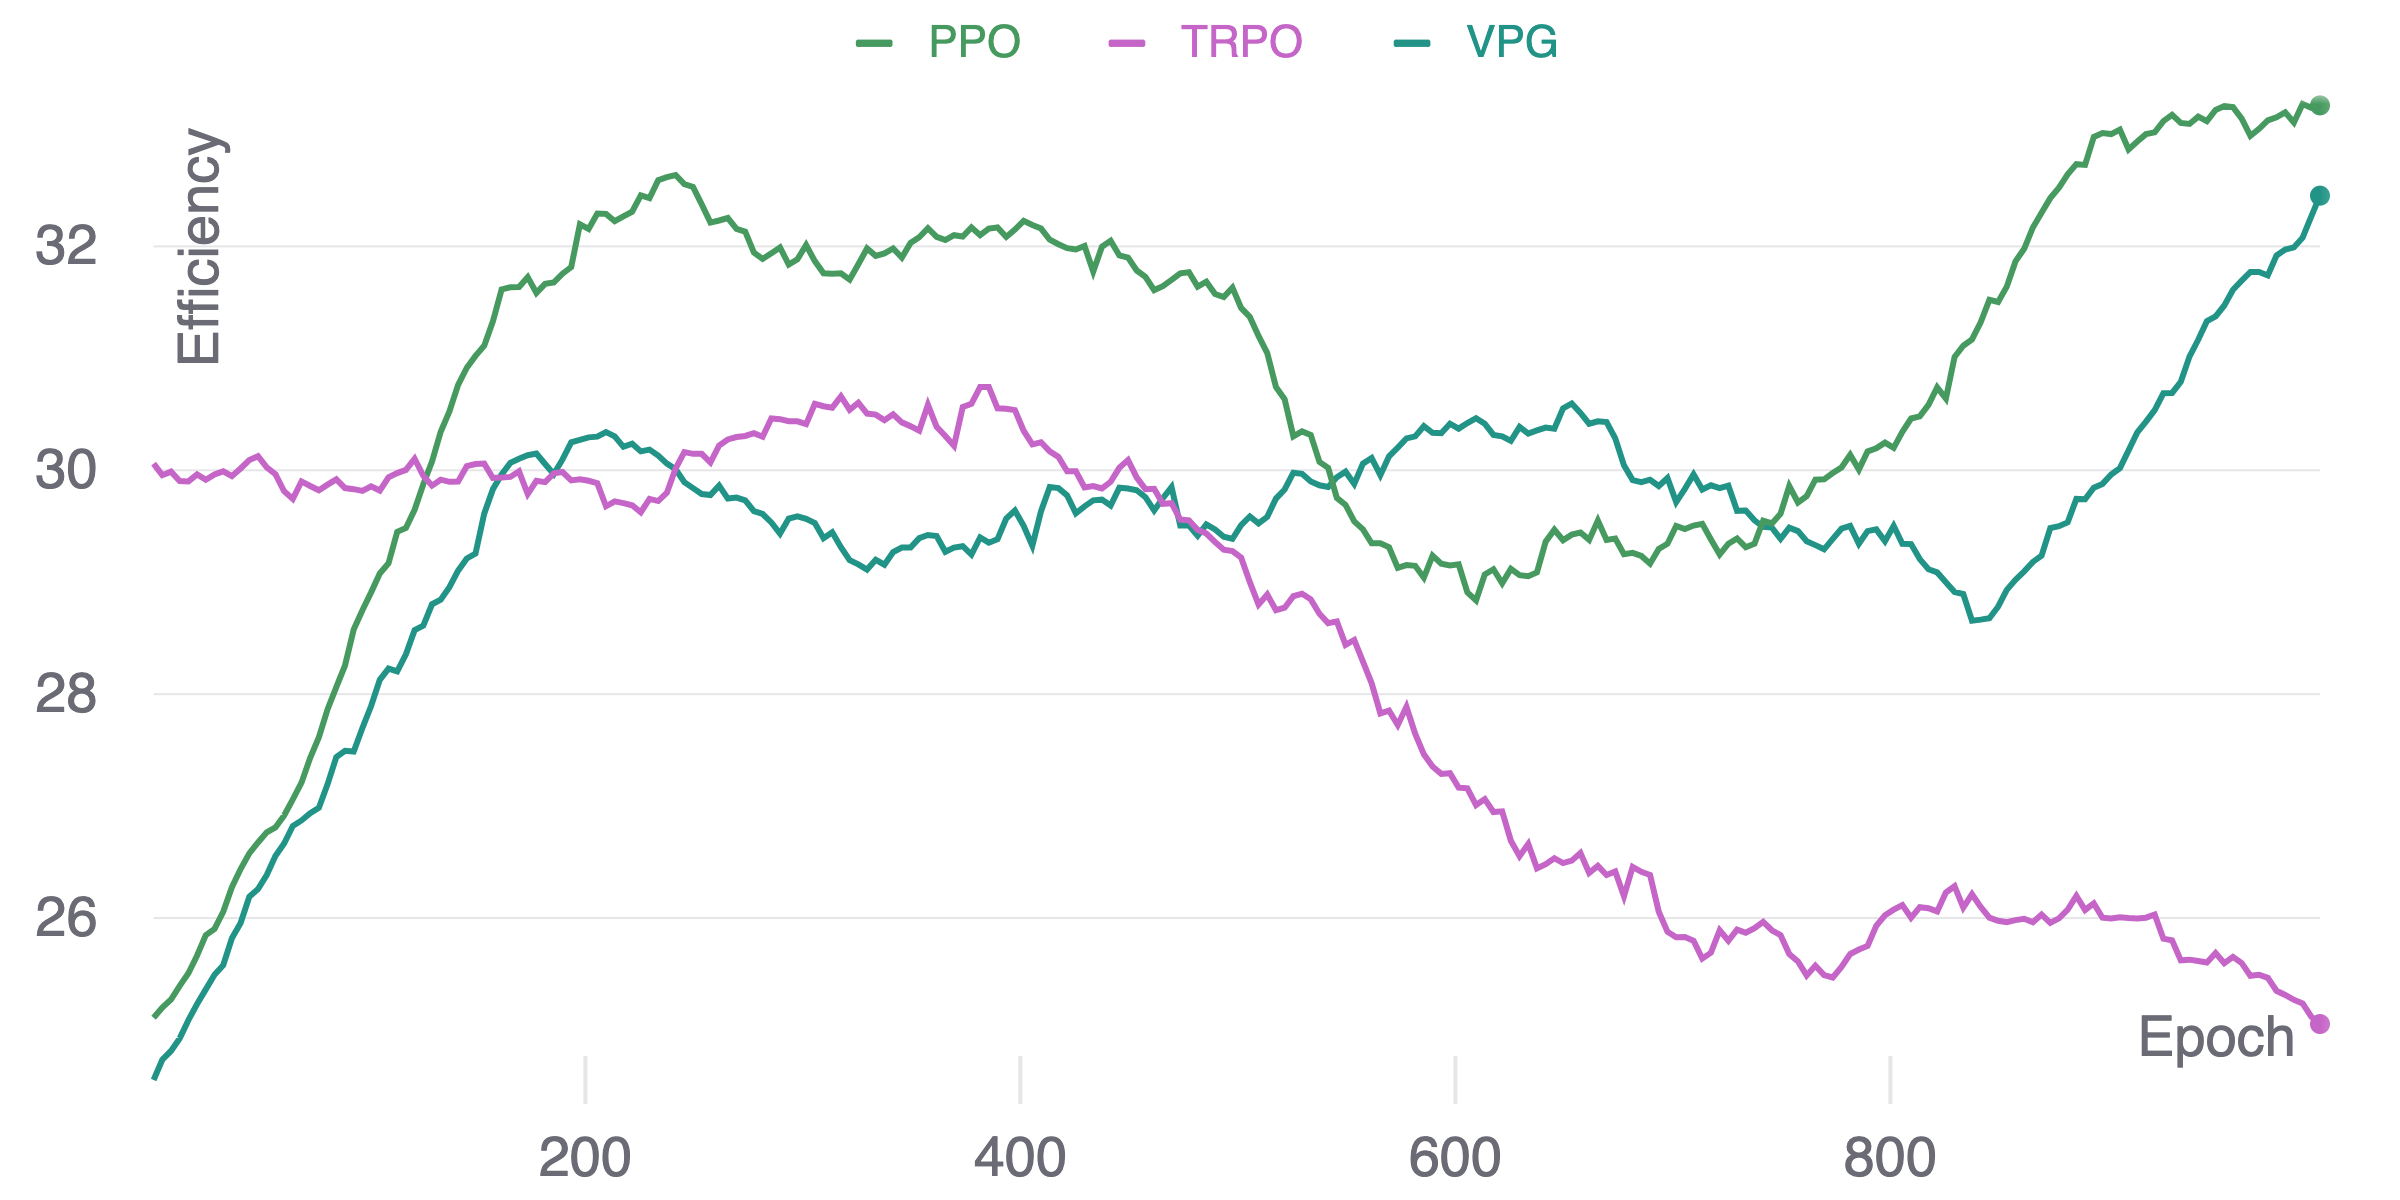
\includegraphics[width=0.9\linewidth]{../assets/vpg-trpo-ppo-single-efficiency.png}
		\caption*{VPG and PPO converge to similar results, while TRPO diverges on the single-agent setting of Harvest}
	\end{figure} 
\end{frame}

\begin{frame}
	\frametitle{Custom PPO on multi-agent Harvest, \\with and without Zero-Sum gifting}
	\begin{figure}
		\centering
		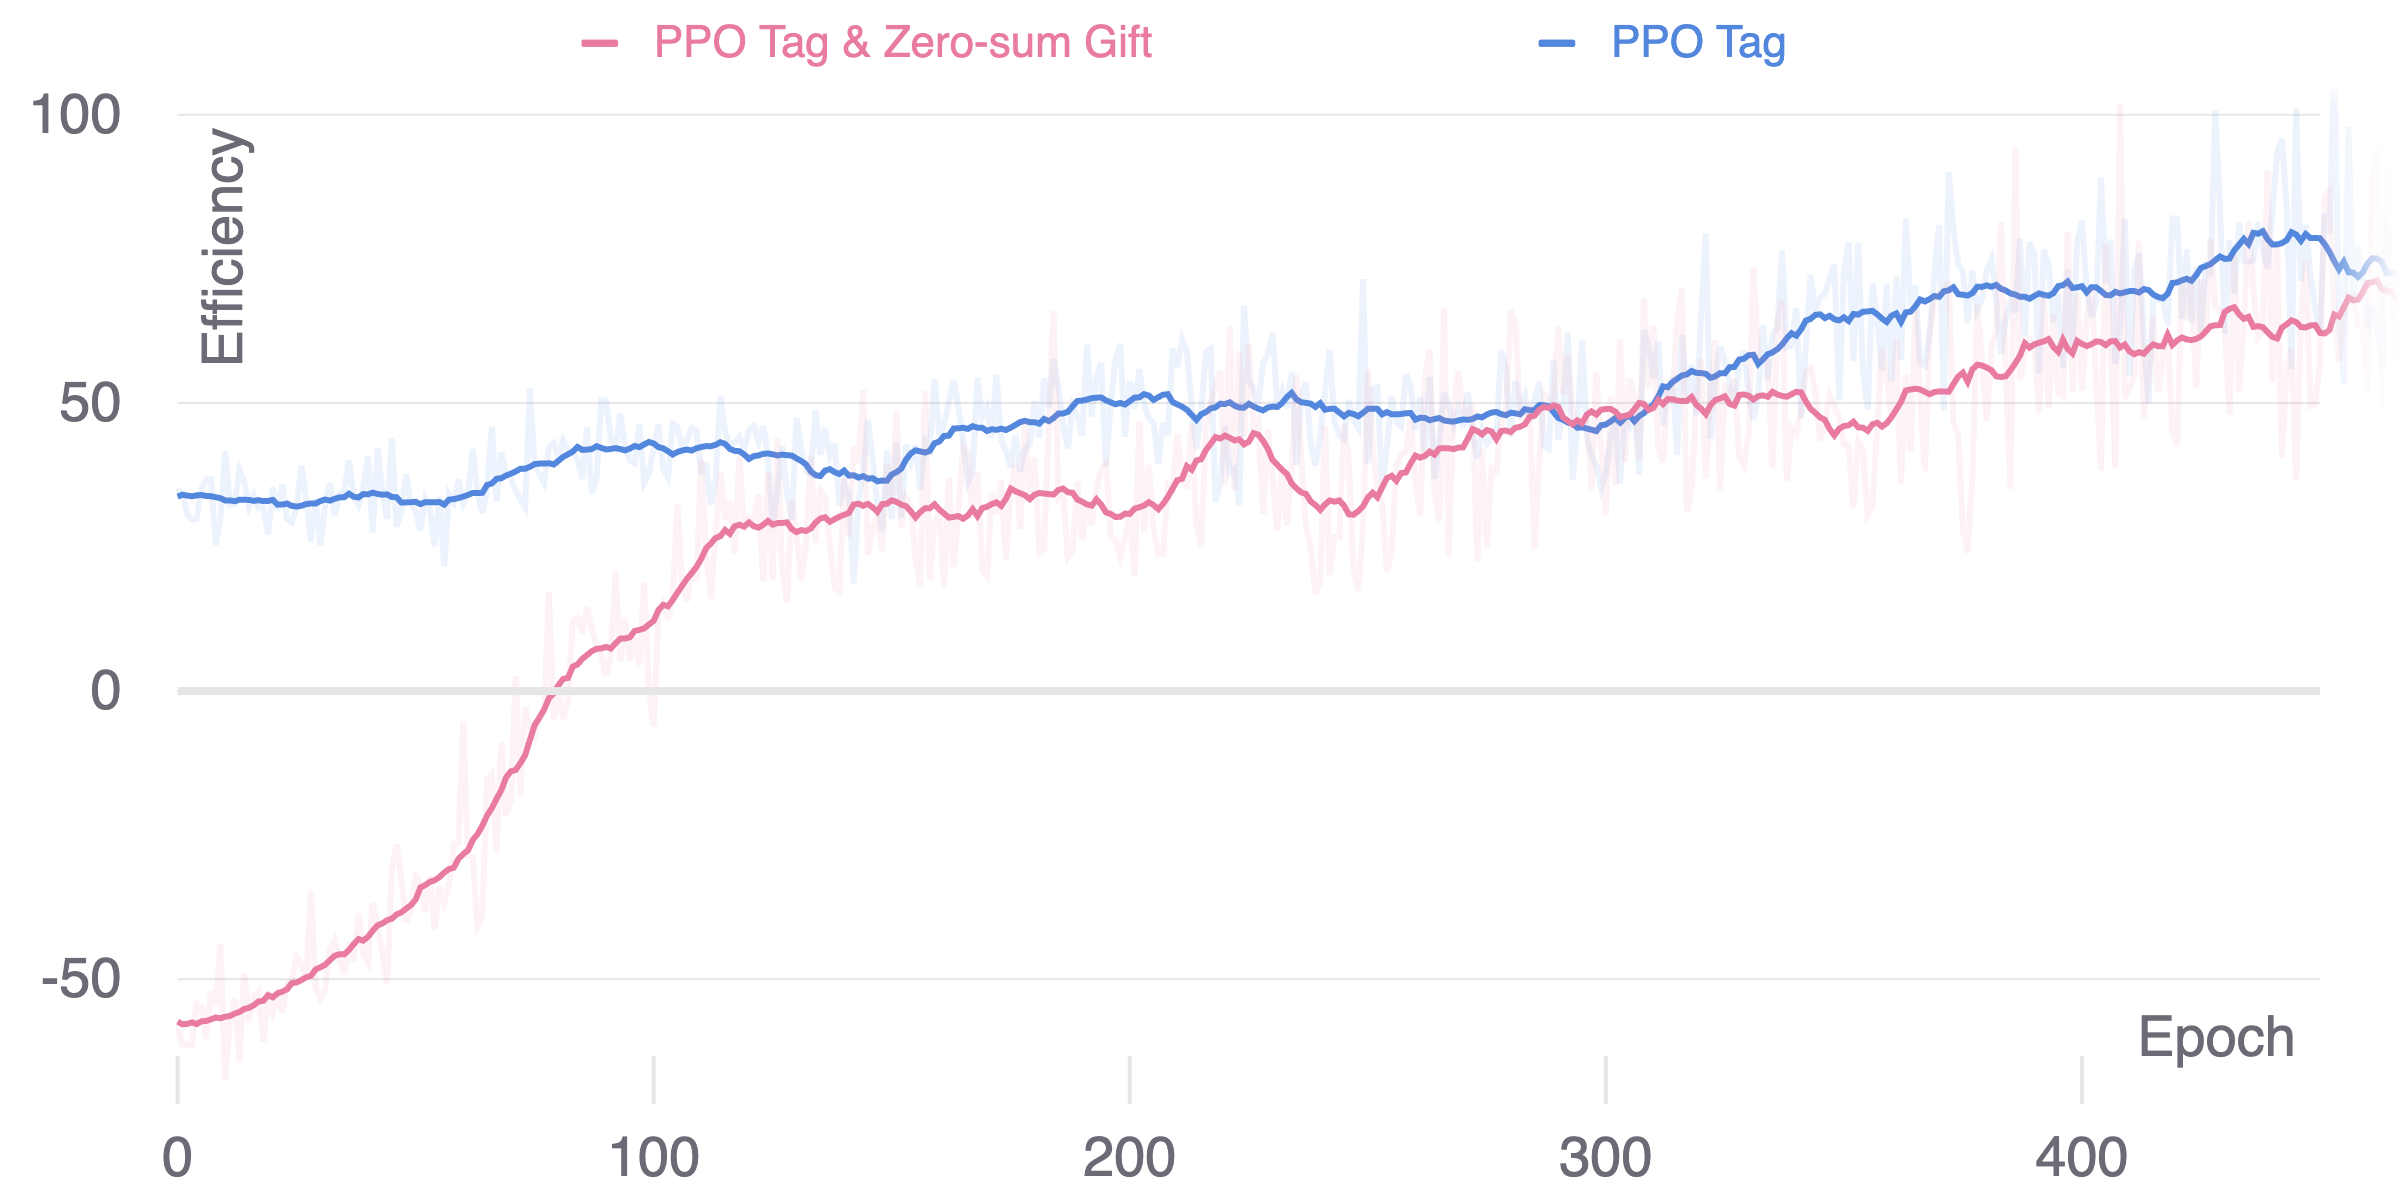
\includegraphics[width=0.9\linewidth]{../assets/ppo-tag-gift-vs-nogift-efficiency.png}
		\caption*{Agents tend to be very generous at the beginning, while later training stages show that enabling or disabling Zero-Sum leads to similar results}
	\end{figure}
\end{frame}

\begin{frame}
	\frametitle{Custom PPO on multi-agent Harvest, \\with Replenishable and Fixed Budget gifting}
	\begin{figure}
		\centering
		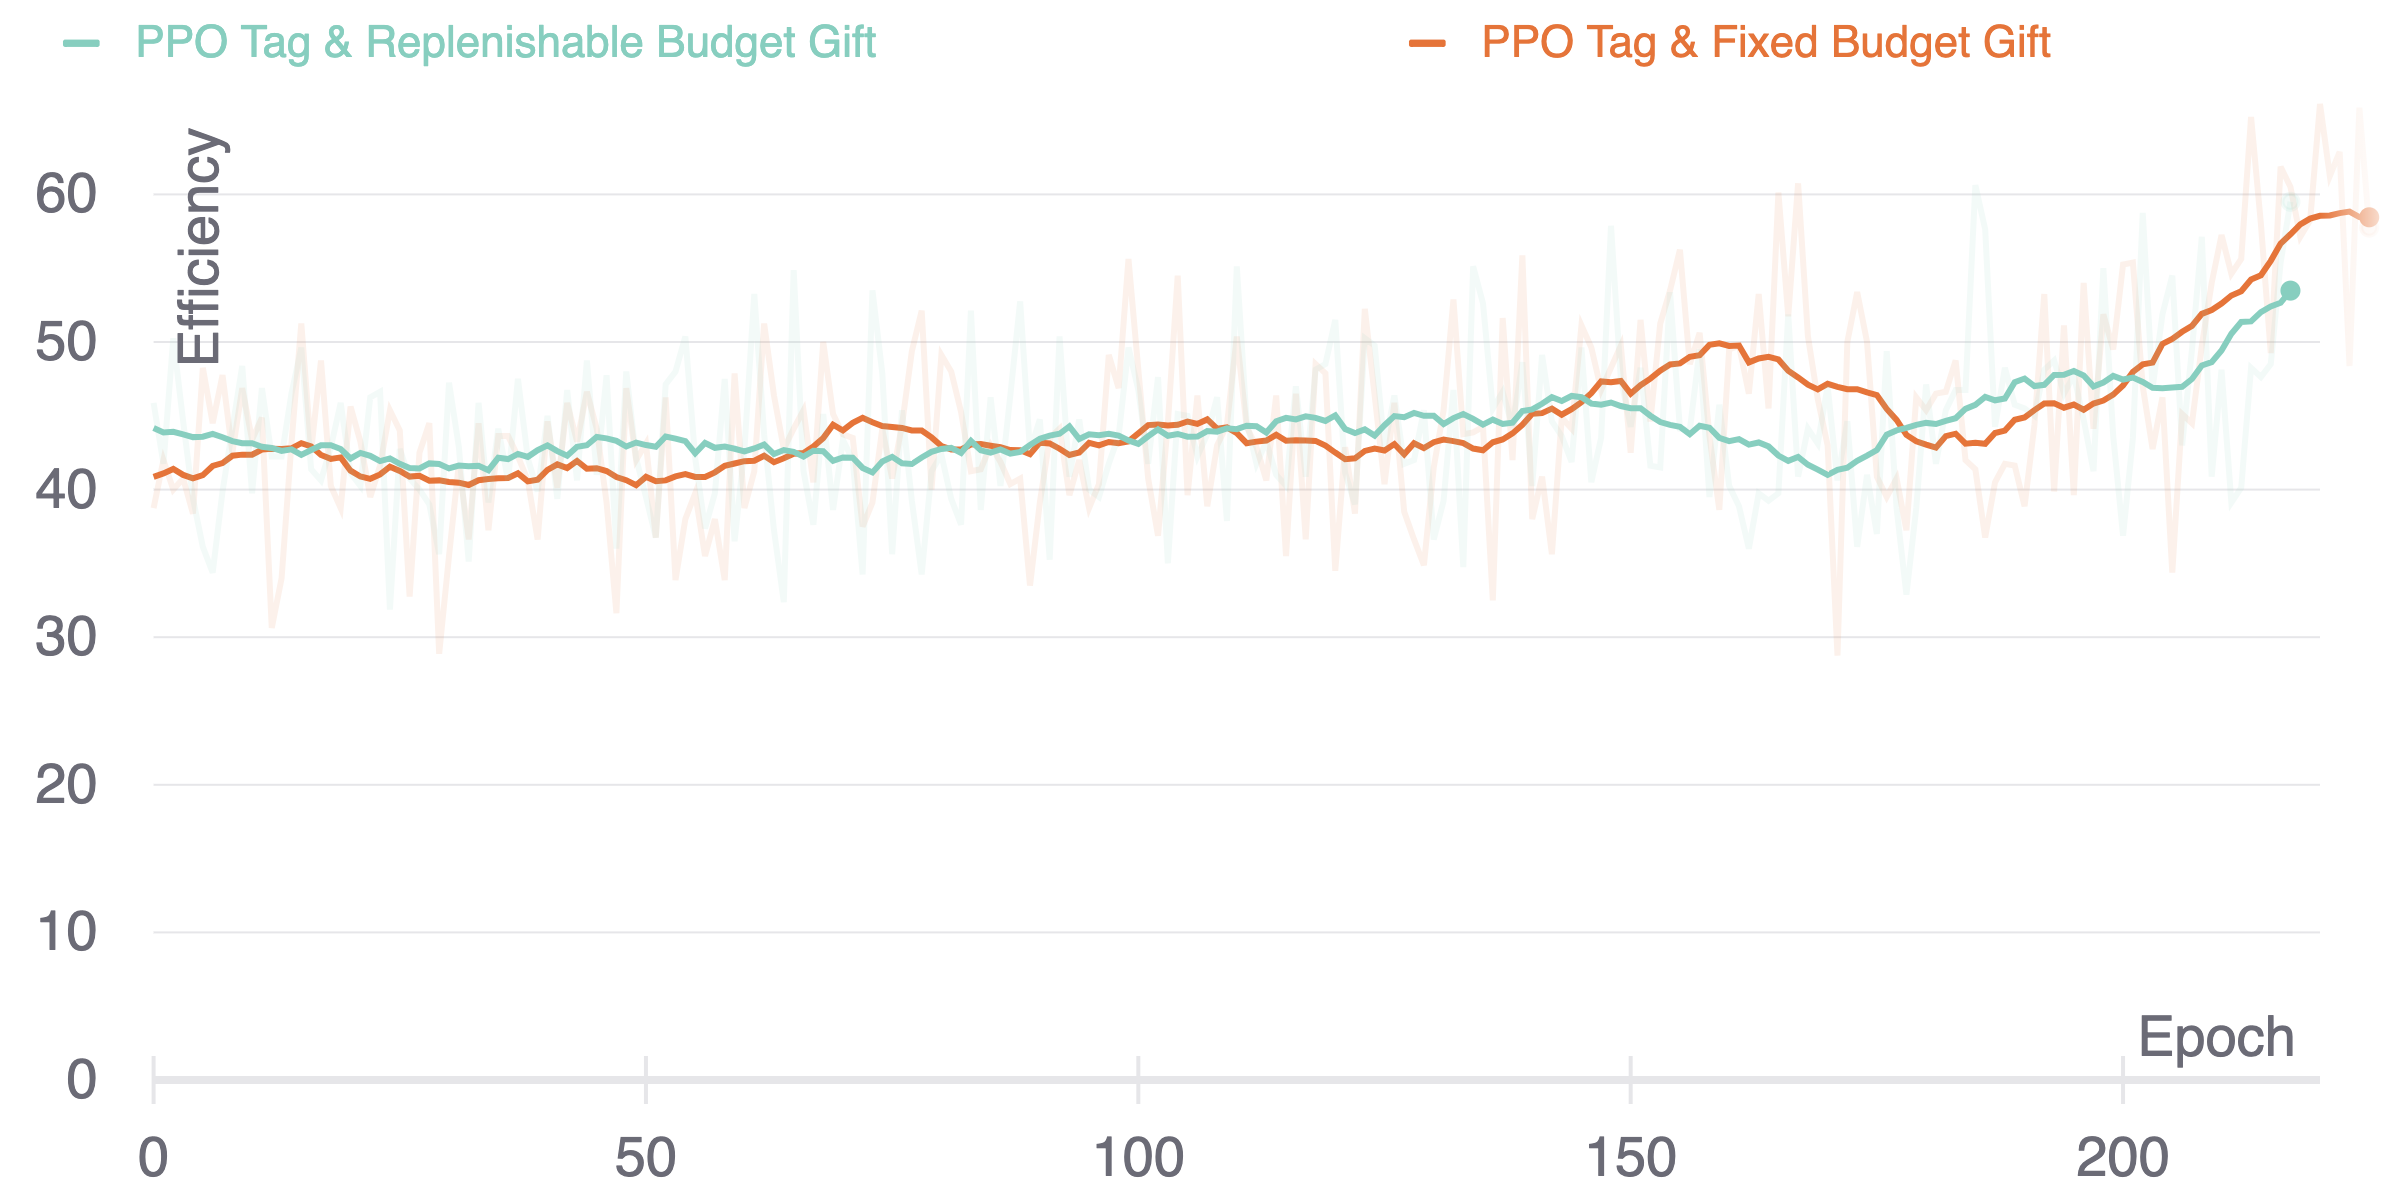
\includegraphics[width=0.9\linewidth]{../assets/ppo-gifting-fixed-vs-replenishable-efficiency.png}
		\caption*{Results show that the Replenishable and Fixed Budget gifting strategies tend to follow similar training curves and converge to comparable results}
	\end{figure}
\end{frame}
\end{document}
